\documentclass[UTF8,a4paper]{ctexart}
\usepackage{xcolor}
\usepackage{graphicx}
\usepackage[margin=1.5in]{geometry}
\usepackage{float}
\usepackage{listings} 
\usepackage{fancyhdr} %用于调整页眉的样式
\usepackage{fancyvrb} 
\usepackage{tabularx}
\usepackage[colorlinks,linkcolor=blue]{hyperref}%用于插入超链接
\usepackage{wallpaper}
\usepackage{tikz}
\usepackage{lipsum}
\usepackage{rotating}
\usepackage{multirow}
\usepackage[absolute]{textpos}
\usetikzlibrary{calc}
\setlength{\TPHorizModule}{1cm}
\setlength{\TPVertModule}{1cm}



\definecolor{color1}{RGB}{10,80,179}
\pagestyle{fancy}
\fancyhead[L]{\url{https://github.com/eric041224/tool_class_2024_sum}}
\setlength{\headheight}{27pt}

\definecolor{GradientTop}{RGB}{0,0,255}
\definecolor{GradientBottom}{RGB}{255,0,0}
\colorlet{GradientMid}{blue!50!red}

\lstset{
    numbers=left,
    numberstyle=\tiny,
    frame=shadowbox,
    rulesepcolor= \color{ red!20!green!20!blue!20},
    escapeinside=``,
    xleftmargin=2em,aboveskip=1em,
    framexleftmargin=2em,
    breaklines=true
}

\hypersetup{
    colorlinks=true,            % 激活链接颜色,去掉链接边框
    urlcolor=color1           % 外部URL链接颜色
}

\begin{document}
%封面
\ThisCenterWallPaper{1.02}{background.png} 
\begin{textblock}{5}(1,2)
    % 设置字号为20pt
    \fontsize{15}{24}\selectfont
    \color{white}
    \begin{turn}{270}
         \qquad 取则行远
        \end{turn}
        \begin{turn}{270}
            海纳百川 
            \end{turn}
    
    \end{textblock}
\begin{center}
    %logo
    \begin{tikzpicture}[remember picture, overlay]
        % 绘制一个矩形,并设置其位置在页面的右上角
        \draw[fill=blue] (current page.north east) rectangle (current page.north west);
        % 在矩形中插入图片,并设置与右上角的距离
        \node[anchor=north east, xshift=-1cm, yshift=-2cm] at (current page.north east) {
            
\includegraphics[width=6cm]{logo.png}
        };
    \end{tikzpicture}

\begin{textblock}{5}(1,24)
    
    \fontsize{120}{24}\selectfont
    \color{color1}
    Week3
       
    
    \end{textblock}

\begin{textblock}{5}(14.5,24)
    
    \fontsize{19}{24}\selectfont
    \color{color1}
    \raggedleft
    左昊天\\
    2024-09-06 \\
    \href{https://github.com/eric041224/tool_class_2024_sum}{Github 仓库地址}\\ 
    
    \end{textblock}

   
\end{center}

\thispagestyle{empty}

\newpage
\color{black}
\section{命令行环境}
\subsection{暂停和后台执行进程}
\begin{table}[H]
    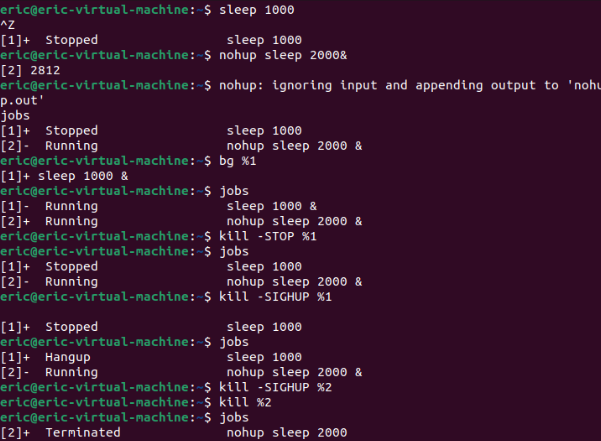
\includegraphics[width=1\textwidth]{./命令行/1.png}
\end{table}
\textbf{解释:}\\
1、sleep 1000 休眠1000s\\
2、control + z 将当前正在运行的前台进程移动到后台,同时暂停该进程的执行\\
3、\verb|&| 将命令放到后台执行\\
4、\verb|bg %1| 恢复第一个任务的执行\\
5、\verb|kill -STOP %1| 暂停第一个任务\\
6、\verb|kill %2| 终止第二个任务

\subsection{我们可以使用类似 ps aux | grep 这样的命令来获取任务的 pid ,然后您可以基于 pid 来结束这些进程。但我们其实有更好的方法来做这件事。在终端中执行 sleep 10000 这个任务。然后用 Ctrl-Z 将其切换到后台并使用 bg 来继续允许它。现在,使用 pgrep 来查找 pid 并使用 pkill 结束进程而不需要手动输入 pid。(提示:: 使用 -af 标记)。}
\begin{table}[H]
    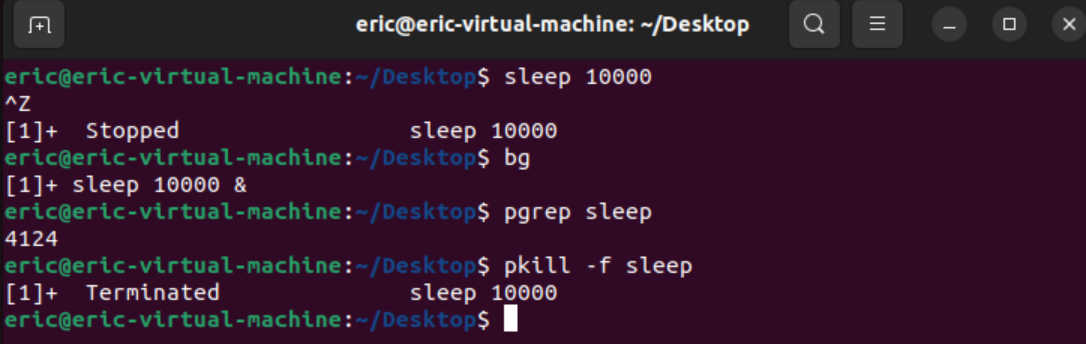
\includegraphics[width=1\textwidth]{./命令行/2.png}
\end{table}
\textbf{解释:}\\
1、pgrep sleep 可以列出包含关键字 sleep 的进程的 pid\\
2、pkill -f sleep 可以终止包含关键字 sleep 的进程

\subsection{终端多路复用}
\textbf{会话:}\\
tmux 开始一个新的会话\\
tmux new -s NAME 以指定名称开始一个新的会话\\
tmux ls 列出当前所有会话\\
在 tmux 中输入 <C-b> d ,将当前会话分离\\
tmux a 重新连接最后一个会话。也可用 -t 来指定具体的会话\par
\textbf{面板:}\\
<C-b> " 水平分割\\
\verb|<C-b> % 垂直分割|\\
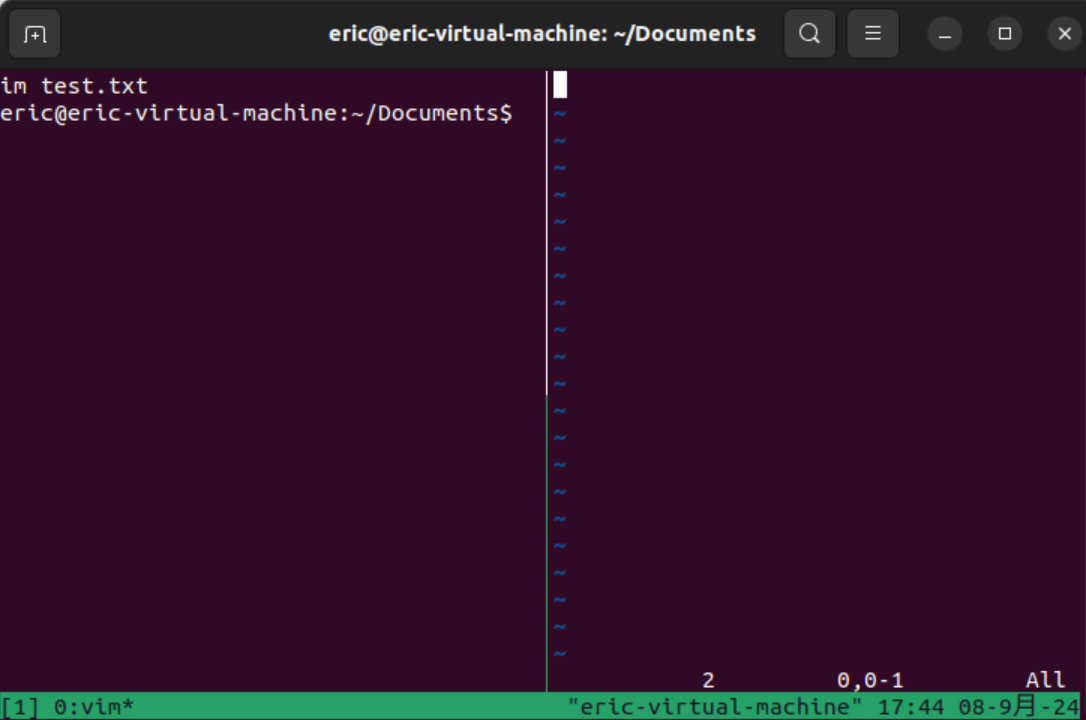
\includegraphics[width=1\textwidth]{./命令行/终端多路复用.png}

\subsection{别名}
\begin{lstlisting}
    alias v="vim"  #用于创建别名
    alias v #用于查看别名的定义
    v 2.txt #使用别名进行操作
    \end{lstlisting}
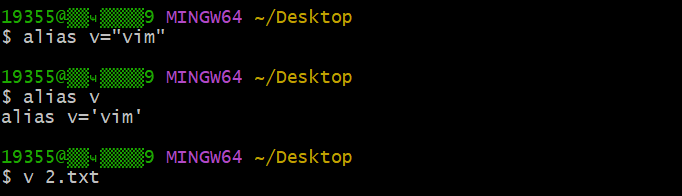
\includegraphics[width=1\textwidth]{./命令行/别名.png}

\subsection{执行以下命令来获取您最常用的十条命令,尝试为它们创建别名。}
命令:
\begin{lstlisting}
    history | awk '{$1="";print substr($0,2)}' | sort | uniq -c | sort -n | tail -n 10 
\end{lstlisting}
\begin{table}[H]
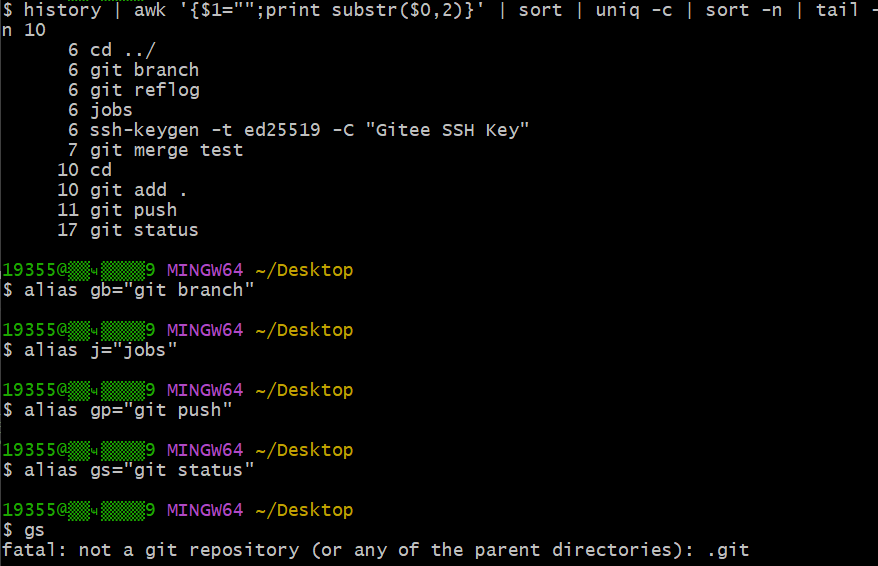
\includegraphics[width=1\textwidth]{./命令行/别名2.png}
\end{table}

\subsection{创建一个 dc 别名,它的功能是当我们错误的将 cd 输入为 dc 时也能正确执行。}
\begin{table}[H]
    
\includegraphics[width=1\textwidth]{./命令行/别名3.png}
\end{table}

\subsection{生成ssh秘钥}
\begin{lstlisting}
    ssh-keygen -o -a 100 -t ed25519 -f ~/.ssh/id_ed25519
\end{lstlisting}
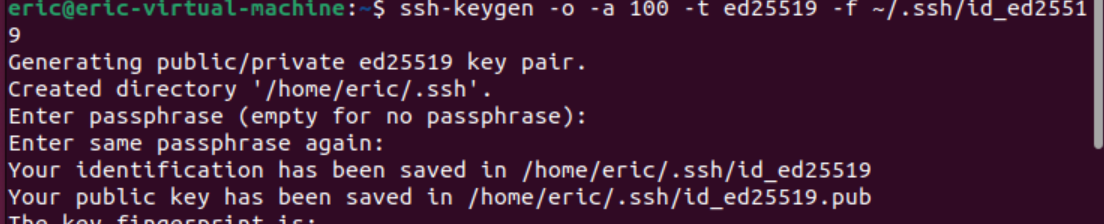
\includegraphics[width=1\textwidth]{./命令行/ssh1.png}

\subsection{ssh配置}
将配置写入.ssh目录下的config文件中\\
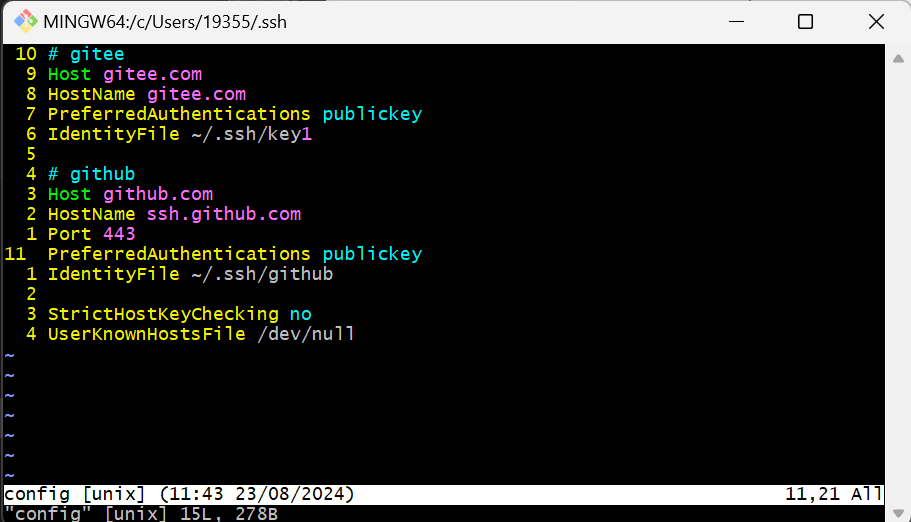
\includegraphics[width=1\textwidth]{./命令行/ssh2.png}

\section{Python基础}
\setcounter{page}{1} %从这开始页面编号
\subsection{输出语句}
\subsubsection{单行输出}
\begin{lstlisting}
print("这是输出的语句")
\end{lstlisting}
print中可以用单引号或双引号,但若想输出的内容中存在同样的引号,会和输出语句的的引号产生歧义。\\
\textbf{解决方法1:}print语句和内容用不同的引号\\
\textbf{解决方法2:}在内容的引号前加转义字符\verb|\|
\begin{lstlisting}
print("I'm fine.")
print('Let\'s go!')
\end{lstlisting}
\subsubsection{多行输出}
使用三引号进行多行输出
\begin{lstlisting}
print('''我相信能再次看到蓝天,
鲜花挂满枝头''')
\end{lstlisting}

\includegraphics[width=1\textwidth]{./python/print1.png}

\subsection{解一元二次方程}
乘方为**  根号可以用**(1/2)或使用math库
\begin{lstlisting}
import math
a=int(input("请输入a的值"))
b=int(input("请输入b的值"))
c=int(input("请输入c的值"))
print((-b+math.sqrt(b**2-4*a*c))/(2*a))
print((-b-math.sqrt(b**2-4*a*c))/(2*a))
\end{lstlisting}

\includegraphics[width=1\textwidth]{./python/math.png}

\subsection{for循环与字典}
\subsubsection{普通循环}
\begin{lstlisting}
total=0
for i in range(1,11):
    total=total+i
print(total)
\end{lstlisting}
\textbf{注:1、python的缩进非常严格,通过缩进判断循环是否结束。}\\
\textbf{2、range的范围左闭右开}\\

\includegraphics[width=1\textwidth]{./python/for1.png}

\subsubsection{对字典的循环}
\begin{lstlisting}
a = {"小王":"123456789","小李":"15462847","小张":"4535415"}
for name,phone in a.items():
    print(name+phone)
\end{lstlisting}

\includegraphics[width=1\textwidth]{./python/for2.png}
\textbf{关于字典:}\\
1、字典是键值对\\
2、a.keys()返回所有键,a.values()返回所有值,a.items()返回所有键值对

\subsection{while循环}
\begin{lstlisting}
i=0
total=0
while i<11:
    total=total+i
    i=i+1
print(total)
\end{lstlisting}

\subsection{格式化字符串}
方法一:
\begin{lstlisting}
name="小王"
print(f"你好{name}")
\end{lstlisting}

方法二:
\begin{lstlisting}
name="小王"
print("你好{0}".format(name))
\end{lstlisting}

\includegraphics[width=1\textwidth]{./python/format.png}

\subsection{函数}
\begin{lstlisting}
def calculate(a):
    s=a*a
    return s
a=float(input("请输入正方形的边长"))
s=calculate(a)
print(f"边长为{a}的正方形的面积为: {s}")
\end{lstlisting}

\includegraphics[width=1\textwidth]{./python/function.png}

\subsection{类}
\subsubsection{创建类以及类的实例化}
\begin{lstlisting}
class Student:
    def __init__(self,name,number,grade): #构造函数
        self.name = name
        self.number = number
        self.grade = grade
    def showStudent(self):
        print("姓名:"+self.name+" 学号:"+self.number+" 年级:"+self.grade)

wang = Student("小王","1","9") #对象的初始化
wang.showStudent()
\end{lstlisting}
\textbf{注:构造函数的下划线是两个下划线并非一个!}\\

\includegraphics[width=1\textwidth]{./python/class.png}
\subsubsection{类的继承}
\begin{lstlisting}
class People:
    def __init__(self,name,age): #构造函数
        self.name = name
        self.age = age

class Student(People):
    def __init__(self,name,age,number,grade): #构造函数
        super().__init__(name,age) 
        self.number = number
        self.grade = grade
    def showStudent(self):
        print("姓名:"+self.name+" 年龄:"+self.age+" 学号:"+self.number+" 年级:"+self.grade)

wang = Student("小王","14","1","9") #对象的初始化
wang.showStudent()
    \end{lstlisting}
\textbf{解释:}\\
1、\verb|super()|会返回当前类的父类,可以用此函数调用父类的构造函数。\\
2、\verb|class Student(People)|中括号的内容表示继承的父类。\\

\includegraphics[width=1\textwidth]{./python/inherit.png}

\subsection{文件的读写}
打开文件的代码:
\begin{lstlisting}
    open("./test.txt","r",encoding="utf-8")
\end{lstlisting}
1、其中第一个引号中表示文件的地址\\
2、第二个引号中表示要对文件进行什么操作\\
3、encoding表示文件的编码方式\\
\begin{table}[H]
    \centering
    \begin{tabular}{c|c}
    第二个引号中的内容 & 可对文件进行的操作\\
    \hline
    r & 只读\\
    w & 只写(覆盖之前的内容)\\
    a & 只写(在已有内容后面添加)\\
    r+ & 读和写(覆盖之前的内容)\\
    a+ & 读和写(追加写)\\
    \hline
\end{tabular}
\end{table}
\subsubsection{文件的读}
.read()返回文件全部内容\par
.readline()返回文件的一行内容\par
.readlines()返回文件所有内容组成的列表\par
\subsubsection{实例}
\begin{lstlisting}
f=open("test.txt","a",encoding="utf-8")
f.write("——— 流浪地球")
f.close()

f=open("test.txt","r",encoding="utf-8")
print(f.read())
f.close()

\end{lstlisting}

\includegraphics[width=1\textwidth]{./python/file1.png}

\section{Python视觉应用}
\subsection{绘制图像、点、线}
\begin{lstlisting}
from PIL import Image
from pylab import *
 # 读取图像到数组中
im = array(Image.open('picture.jpg'))
 # 绘制图像
imshow(im)
 # 一些点
x = [100,100,400,400]
y = [200,500,200,500]
 # 使用红色星状标记绘制点
plot(x,y,'r*')
 # 绘制连接前两个点的线
plot(x[:2],y[:2])
 # 添加标题,显示绘制的图像
title('Plotting: "picture.jpg"')
show()
\end{lstlisting}
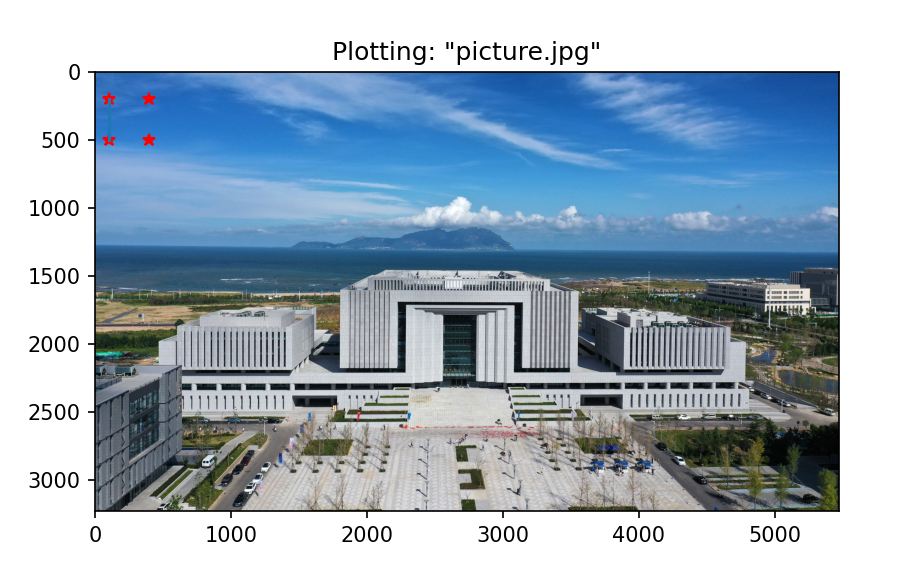
\includegraphics[width=1\textwidth]{./python/visual4.png}

\subsection{创建缩略图}
\begin{lstlisting}
import matplotlib.pyplot as plt
from PIL import Image

pil_im = Image.open('picture.jpg')
pil_im.thumbnail((128,128))
plt.imshow(pil_im)
plt.axis('off')
plt.show()
\end{lstlisting}
原图片:\\
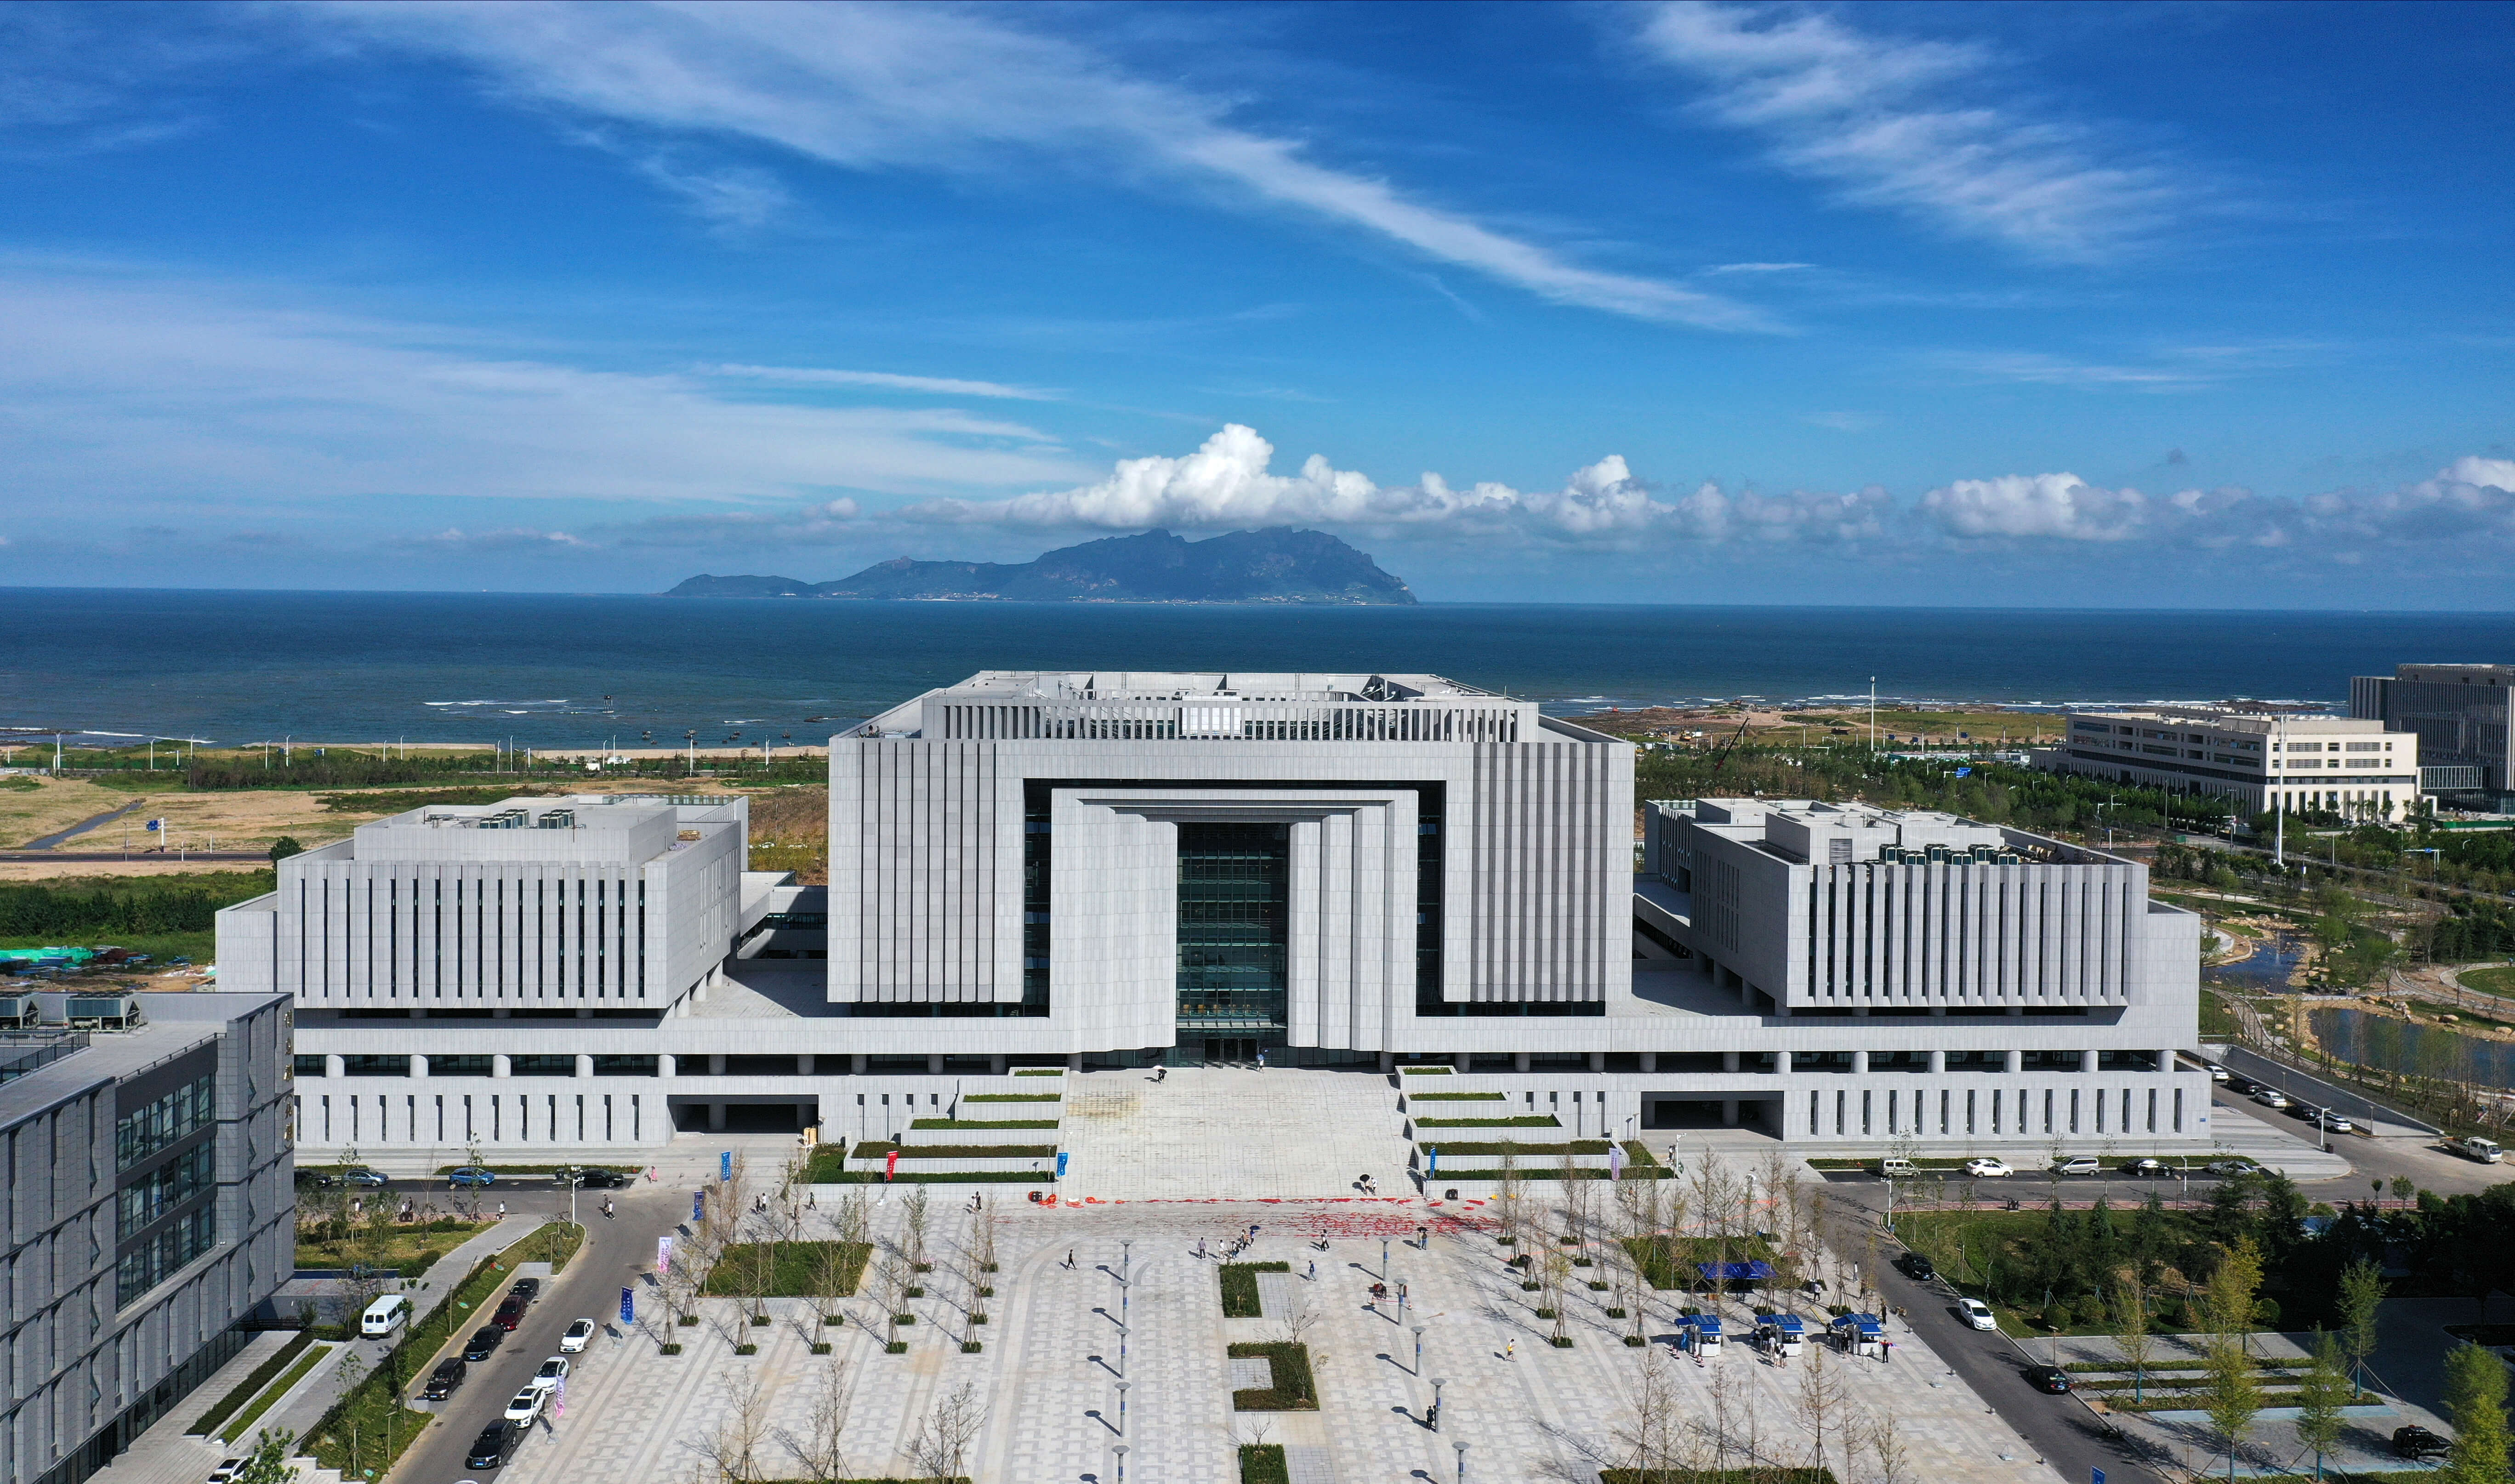
\includegraphics[width=1\textwidth]{./python/picture.jpg}\\
创建的缩略图:\\
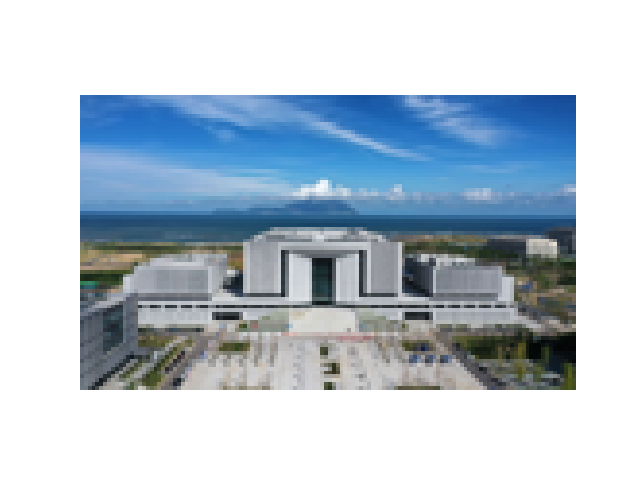
\includegraphics[width=1\textwidth]{./python/缩略图.png}
\subsection{生成图像轮廓和直方图}
\begin{lstlisting}
from PIL import Image
from pylab import *
 # 读取图像到数组中
im = array(Image.open('picture.jpg').convert('L'))
 # 新建一个图像
figure()
 # 不使用颜色信息
gray()
 # 在原点的左上角显示轮廓图像
contour(im, origin='image')
axis('equal')
axis('off')
figure()
hist(im.flatten(),128)
show()
\end{lstlisting}
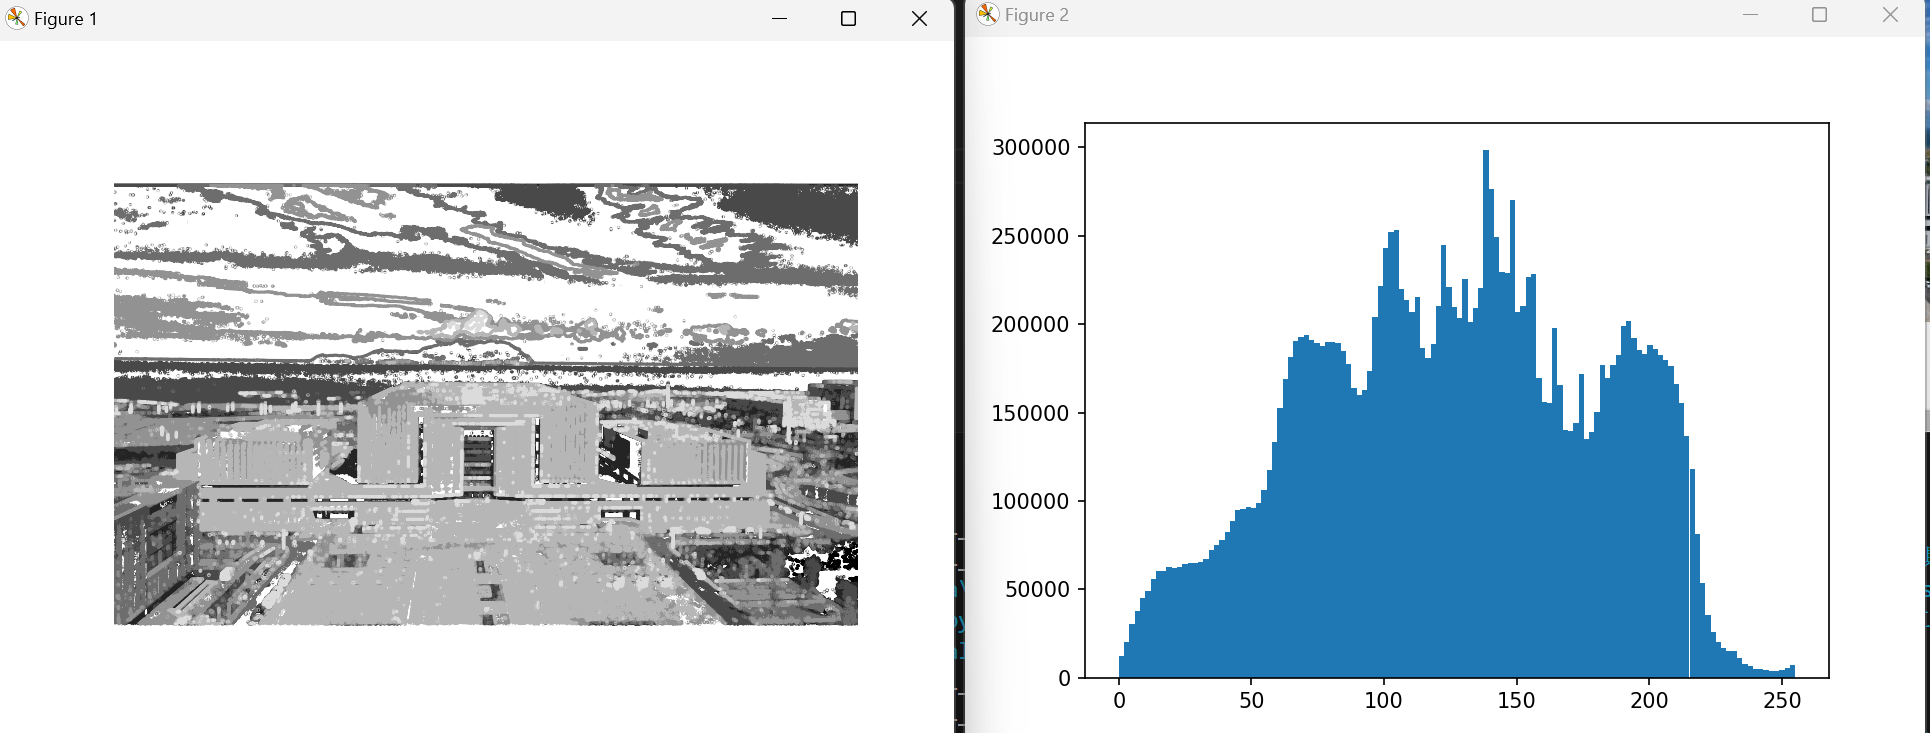
\includegraphics[width=1\textwidth]{./python/visual2.png}
\textbf{遇到的问题:}vs code中的python无法识别相对路径\\
\textbf{解决方法:}在launch.json配置文件中添加\verb|"cwd": "${fileDirname}"|

\subsection{交互式批注}
在绘图窗口的图像区域点击三次,程序将这些点击的坐标[x, y]自动保存在x列表里。
\begin{lstlisting}
from PIL import Image
from pylab import *
im = array(Image.open('picture.jpg'))
imshow(im)
print ('Please click 3 points')
x = ginput(3)
print ('you clicked:',x)
show()
\end{lstlisting}
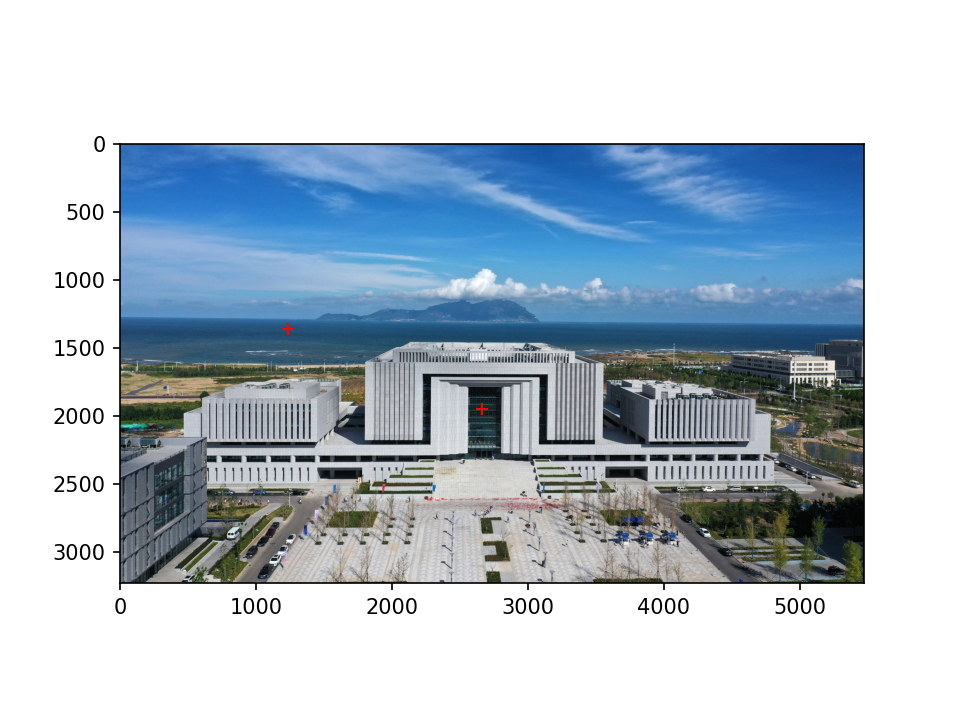
\includegraphics[width=1\textwidth]{./python/visual3-1.png}\\
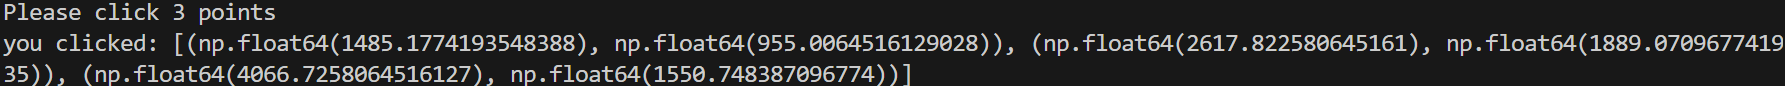
\includegraphics[width=1\textwidth]{./python/visual3-2.png}
\end{document}
